\paragraph{V4 - Rust}

Die V4 Variante wird ebenfalls in Rust entwickelt, aber von Grund auf neu aufgebaut. Die Architektur wird komplett überarbeitet und stark vereinfacht. Die \Gls{statemachine} wird verworfen und die ganze Applikation basiert auf dem Datenbank \Gls{listener}. Der Listener wird mithilfe Funktionalität der \texttt{firestore\_rs} (\ref{sec:firestore_rs}) Softwarebilbiothek implementiert.

\subparagraph{Projektstruktur}

Das Projekt wird mit dem command \texttt{cargo new} erstellt, deshalb ist die Projektstruktur wie folgt:

\dirtree{%
  .1 tower\_controller\_v4.
  .2 src.
  .3 bin.
  .3 entities.
}

\begin{itemize}
  \item \textbf{\texttt{tower\_controller\_v4}} Root Verzeichnis des Projekts, hier befinden sich alle    Konfigurationsdateien (Cargo.toml, Cargo.lock, .gitignore, etc\ldots{}).
  \item \textbf{\texttt{src}} Hier befinden sich alle Quellcode Dateien.
  \item \textbf{\texttt{bin}} Hier befinden sich alle Quellcode Dateien, die ausgeführt werden können.
  \item \textbf{\texttt{entities}} Hier befinden sich die serialisierbaren Datenstrukturen (Entities), die den Dokumenten in der Datenbank entsprechen.
\end{itemize}

\subparagraph{Programmablauf}
\begin{enumerate}
  \item Der Turm Controller wird mittels der \texttt{main} Funktion gestartet.
  \item Umgebungsvariablen werden geladen.
  \item Datenbank Interface wird erstellt (\texttt{TowerDatabase::new}).
  \item Turm Datenstruktur wird erstellt und mit den Daten aus der Datenbank initialisiert\\(\texttt{Tower::new}).
  \item Assignment Scheduler wird erstellt (\texttt{AssignmentScheduler::new}).
  \item Der Scheduler wird gestartet (\texttt{AssignmentScheduler::start}) und der main \Gls{thread} wird in den \Gls{sleep} Modus versetzt.
  \item Das Programm wartet nun auf Änderungen in der Datenbank.
\end{enumerate}

\begin{figure}[H]
  \centering
  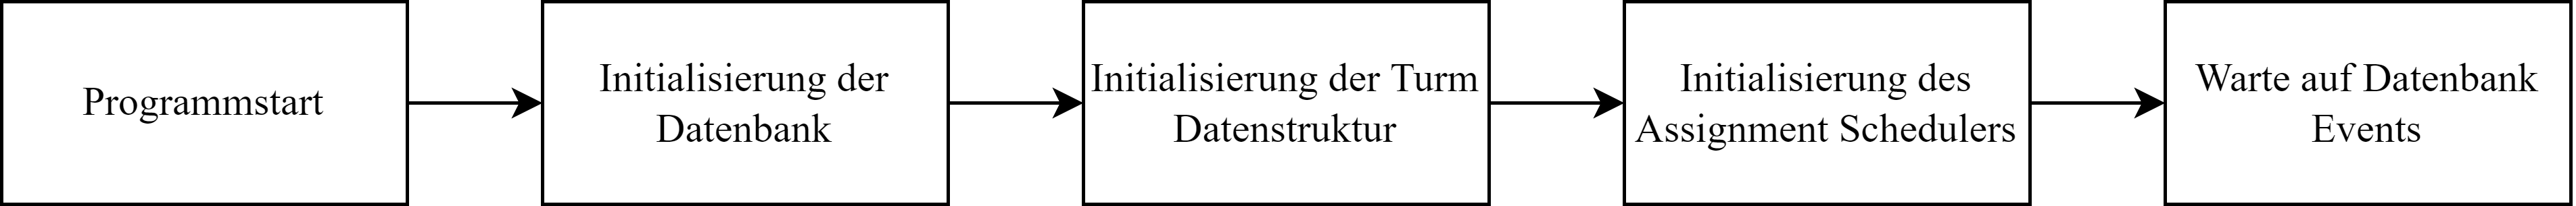
\includegraphics[width=1\textwidth]{images/tower_controller_v4_init.png}
  \caption{Intialisierung des Turm Controllers}
  \label{fig:tower_controller_v4_init}
\end{figure}

\clearpage

\subparagraph{Event Handling Pipeline}

Wenn der Turm Controller ein Event empfängt, wird dieses in der Event Handling Pipeline verarbeitet. Die Event Handling Pipeline besteht aus Validierungs- und Ausführungsstufen. Die Validierungsstufen prüfen, ob das Event gültig ist und ob es überhaupt verarbeitet werden muss. Die Ausführungsstufen führen die eigentliche Verarbeitung des Events aus. Die Funktionsweise der Event Handling Pipeline ist in Abbildung \ref{fig:tower_controller_v4_event_handling} dargestellt.

\begin{figure}[H]
  \centering
  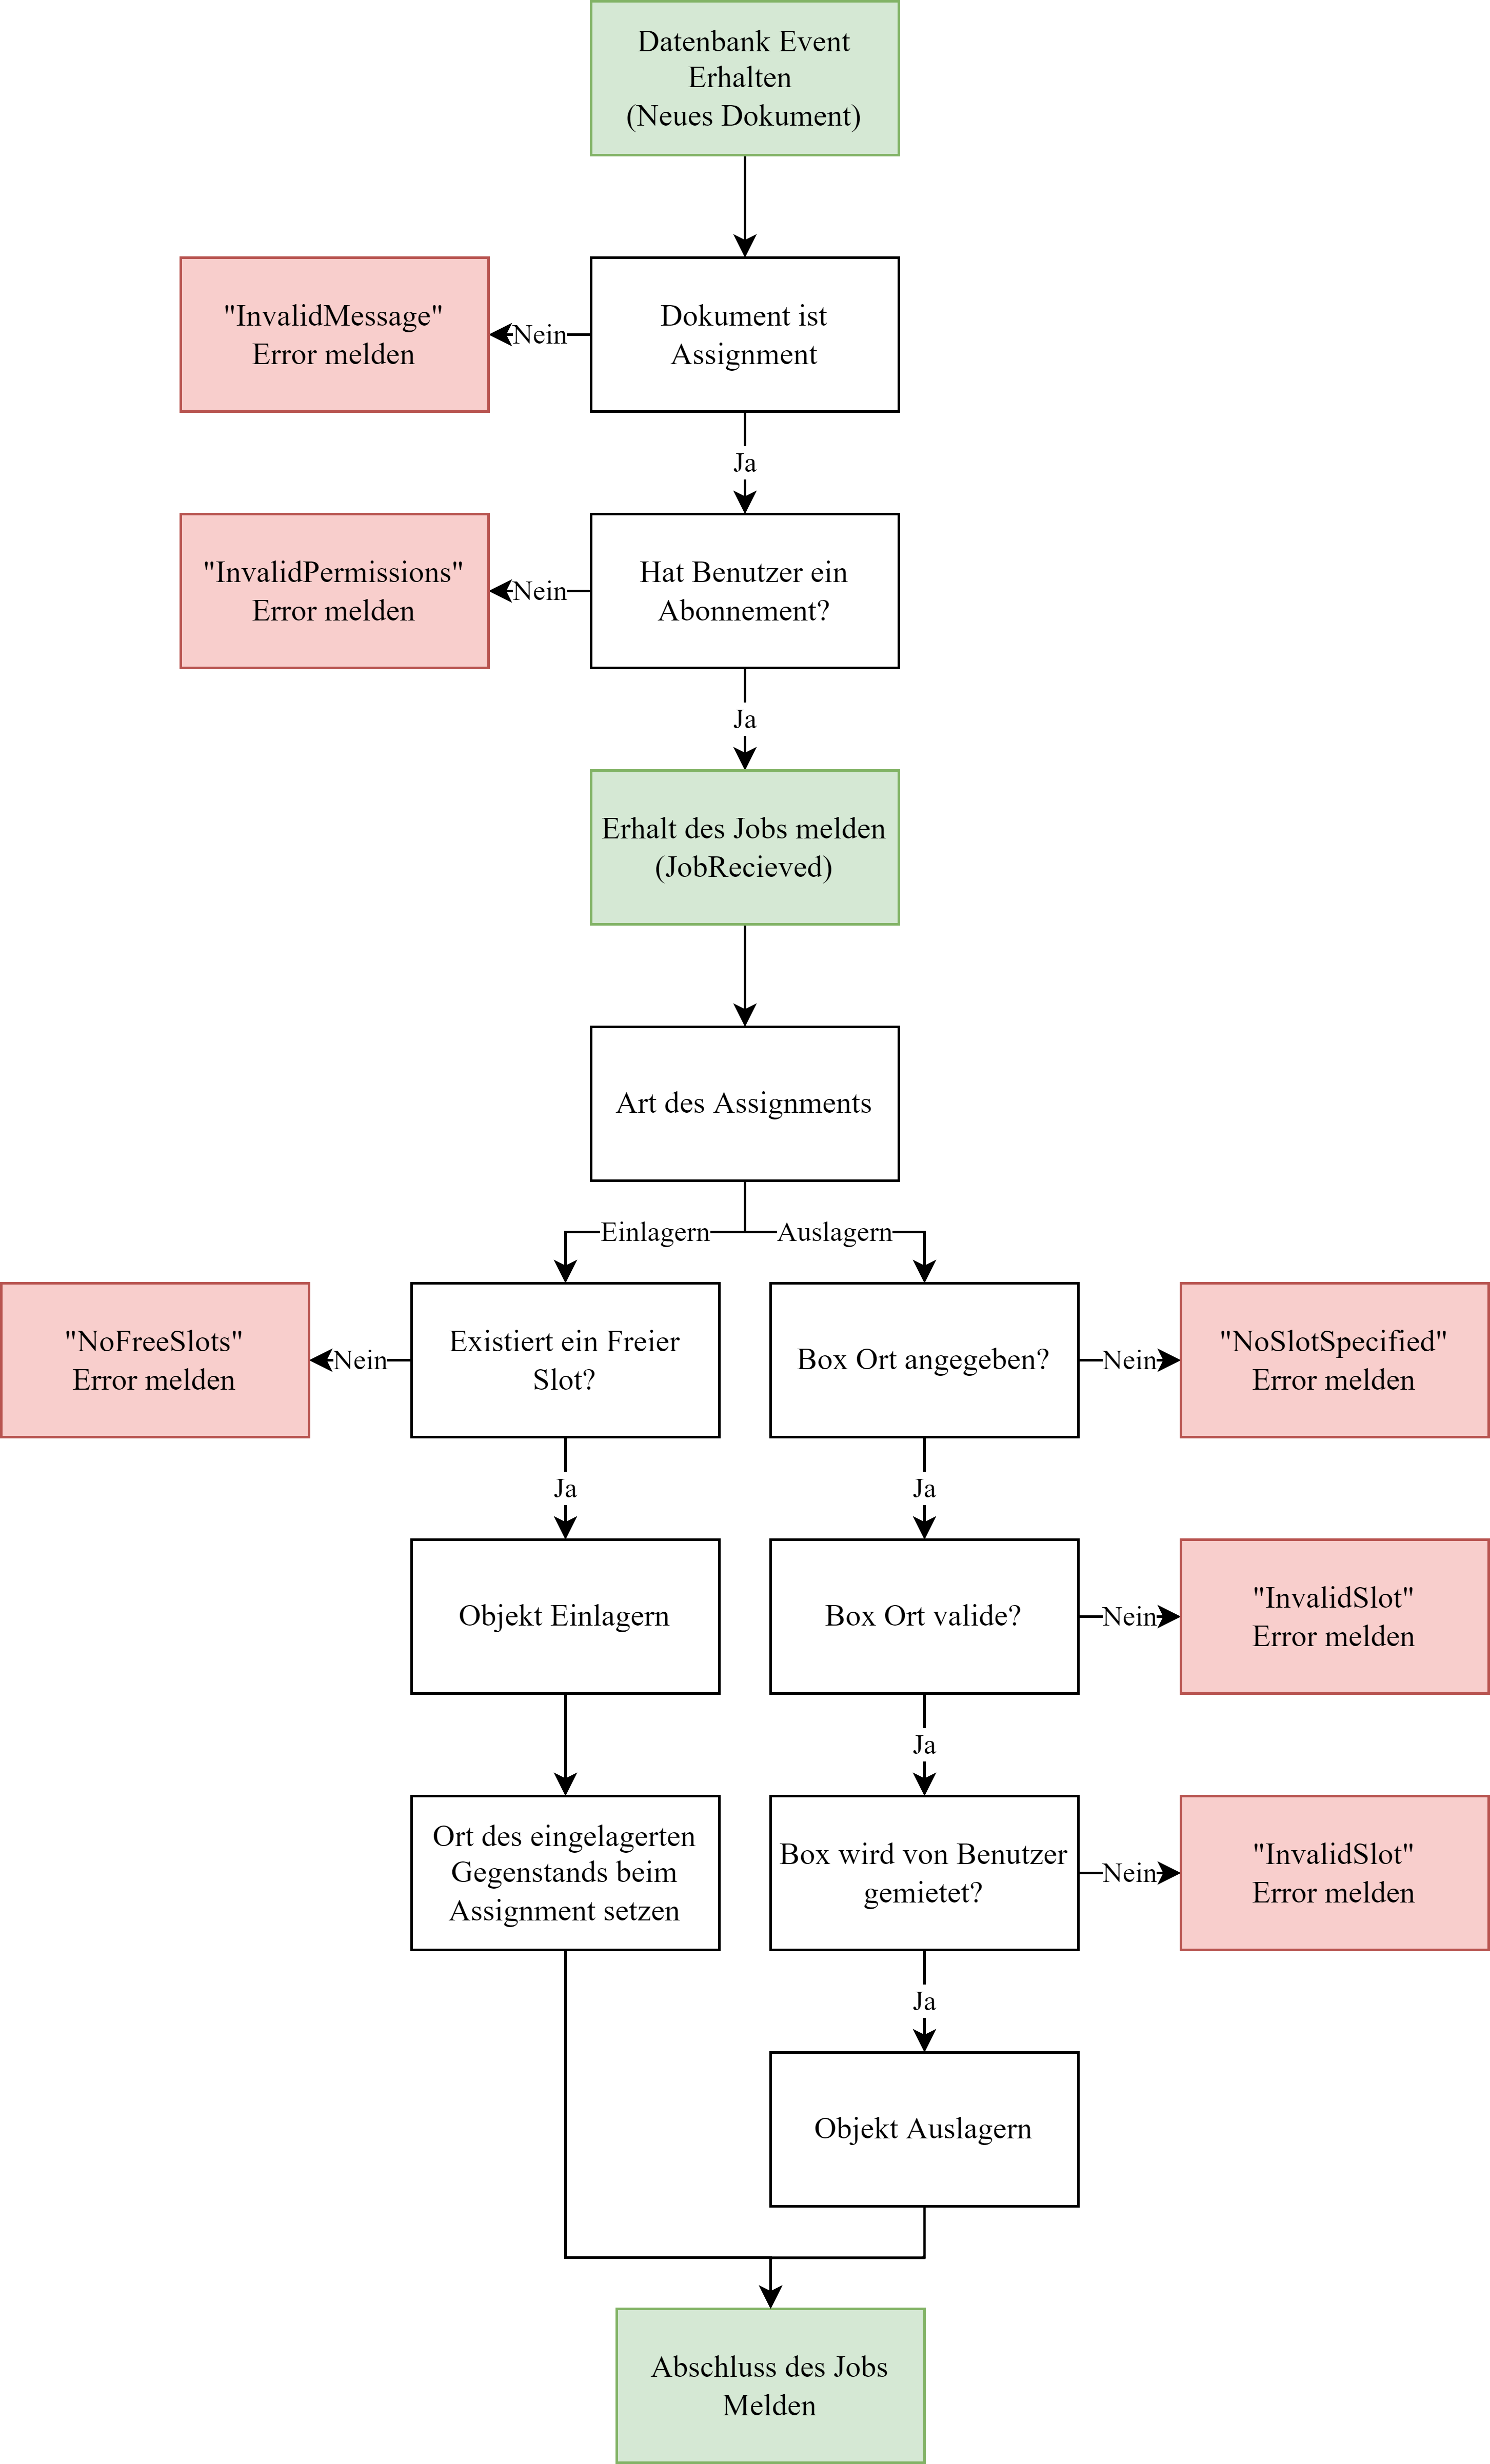
\includegraphics[width=0.6\textwidth]{images/tower_controller_v4_event_handling.png}
  \caption{Event Handling Pipeline}
  \label{fig:tower_controller_v4_event_handling}
\end{figure}

In Abbildung \ref{fig:tower_controller_v4_event_handling} werden nicht alle möglichen Fehler dargestellt sondern nur welche, für die der Benutzer der \ac{API} verantwortlich ist. Fehler, welche aufgrund eines internen Fehlers auftreten, werden nicht dargestellt (Fehler bei Datenbankverbindung, Programmlogikfehler, etc...).

\clearpage

\subparagraph{TowerDatabase}

\texttt{TowerDatabase} kümmert sich um die Kommunikation mit der Datenbank. Es ist ein \Gls{wrapper} für die Datenbankverbindung der \texttt{firestore\_rs} Softwarebilbiothek.
Es vereinfacht die Interaktion mit der Datenbank und minimiert die möglichekeit von Fehlern.

\begin{listing}[H]
  \begin{minted}{rust}
struct TowerDatabase {
    db: FirestoreDb,
    tower_id: String,
    project_id: String,
}
  \end{minted}
  \caption{TowerDatabase Struktur}
  \label{lst:tower_database_struktur}
\end{listing}

\textbf{Felder:}
\begin{itemize}
  \item \textbf{\texttt{db}}: Datenbankverbindung.
  \item \textbf{\texttt{tower\_id}}: ID des Turms.
  \item \textbf{\texttt{project\_id}}: ID des Projekts.
\end{itemize}

\textbf{Methoden:}
\begin{itemize}
  \item \textbf{\texttt{new}}: Erstellt eine neue Instanz von \texttt{TowerDatabase}.
  \item \textbf{\texttt{has\_subscription}}: Prüft, ob ein nutzer eine Abonnement hat.
  \item \textbf{\texttt{set\_error}}: Setzt einen Fehlerstatus eines Assignments.
  \item \textbf{\texttt{set\_confirm}}: Setzt einen Bestätigungsstatus eines Assignments.
  \item \textbf{\texttt{set\_slot}}: Setzt einen Slot eines Assignments.
  \item \textbf{\texttt{create\_listener}}: Erstellt einen Listener, welcher auf Änderungen in der \texttt{jobs} Collection wartet.
  \item \textbf{\texttt{get\_tower}}: Lädt die Daten des Turms aus der Datenbank (Wichtig für die Initialisierung des Turms).
  \item \textbf{\texttt{create\_boxes}}: Erstellt fehlende Boxen in der Datenbank anhand des Layout Feldes im Turm Dokument.
  \item \textbf{\texttt{new\_rental}}: Erstellt einen neuen Mietvorgang in der Datenbank (users > rentals).
  \item \textbf{\texttt{finish\_rental}}: Beendet einen Mietvorgang in der Datenbank.
\end{itemize}


\subparagraph{Tower}

\texttt{Tower} ist die Datenstruktur des Turms. Sie enthält alle Informationen über den Turm und die Boxen. Sie wird vom \texttt{AssignmentScheduler} verwendet, um die Boxen zu verwalten. Tower enthält zusätzlich Methoden um die Datenstruktur zu verwalten.

\begin{listing}[H]
  \begin{minted}{rust}
struct Tower {
    id: String,
    slots: HashMap<Vec<u32>, Slot>,
    layout: Vec<u32>,
    db: Arc<TowerDatabase>,
}
\end{minted}
  \caption{Tower Struktur}
  \label{lst:tower_struktur}
\end{listing}

\textbf{Felder:}
\begin{itemize}
  \item \textbf{\texttt{id}}: ID des Turms.
  \item \textbf{\texttt{slots}}: Alle Slots des Turms. Der Schlüssel ist ein Vektor (Dynamischer Array) an \texttt{u32} Werten, welche die Position der Boxen im Turm beschreiben.
  \item \textbf{\texttt{layout}}: Layout des Turms.
  \item \textbf{\texttt{db}}: Datenbankverbindung (\texttt{Arc<T>} als \Gls{wrapper} um Referenzen in mehreren \Glspl{thread} zu erlauben).
\end{itemize}

\textbf{Methoden:}
\begin{itemize}
  \item \textbf{\texttt{new}}: Erstellt eine neue Instanz von \texttt{Tower}.
  \item \textbf{\texttt{find\_free\_slot}}: Sucht einen freien Slot für ein Assignment.
  \item \textbf{\texttt{store\_object}}: Speichert ein Objekt (Fahrrad) in einer Box.
  \item \textbf{\texttt{retrieve\_object}}: Entfernt ein Objekt (Fahrrad) aus einer Box.
  \item \textbf{\texttt{slot\_exitst}}: Prüft ob ein Slot existiert.
  \item \textbf{\texttt{slot\_rented\_by\_user}}: Prüft ob ein Slot von einem bestimmten Nutzer gemietet ist.
  \item \textbf{\texttt{rent\_box}}: Mietet eine Box.
        \item\textbf{\texttt{unrent\_box}}: Beendet die Miete einer Box.
\end{itemize}


\subparagraph{AssignmentScheduler}

Der AssignmentScheduler hört auf Datenbankevents und verarbeitet diese.

\begin{listing}[H]
  \begin{minted}{rust}
pub struct AssignmentScheduler {
    db: Arc<TowerDatabase>,
    tower: Arc<Mutex<Tower>>,
    listener: FirestoreListener<FirestoreDb, HashMapTokenStorage>,
}
\end{minted}
  \caption{AssignmentScheduler Struktur}
  \label{lst:assignment_scheduler_struktur}
\end{listing}

\textbf{Felder:}
\begin{itemize}
  \item \textbf{\texttt{db}}: Datenbankverbindung.
  \item \textbf{\texttt{tower}}: Turm (Der \texttt{Mutex<T>} erlaubt das paralelle Ändern von Daten ohne \glspl{racecondition} zu erzeugen).
  \item \textbf{\texttt{listener}}: Listener für die \texttt{jobs} Collection.
\end{itemize}

\textbf{Methoden:}
\begin{itemize}
  \item \textbf{\texttt{new}}: Erstellt eine neue Instanz des \texttt{AssignmentScheduler}.
  \item \textbf{\texttt{listen}}: Startet den Listener.
  \item \textbf{\texttt{stop}}: Stoppt den Listener.
\end{itemize}


\subparagraph{TowerDisplay}

Der TowerDisplay ist für die Anzeige mittels der LEDs zuständig. Er wird von der \texttt{Tower} Klasse verwendet, um den momentanen Zustand des Turms anzuzeigen.

Als erstes wird der Zustand des Turms zu einem langen hexadezimal String umgewandelt. Dieser String wird dann an ein kleines Python Script übergeben, welches die LEDs ansteuert. Das Python Script wird verwendet da es einfacher ist, die LEDs mit Python anzusteuern als mit Rust.